\subsection{Quantitative analysis}

We use 21,207 SO snippets as our query code base and get their similar counterparts in GitHub. 
The SO snippets have a median of two GitHub clones and a mean of one GitHub clones. The distribution of number of GitHub clones is shown in Figure \ref{fig:num-clone}. From the distribution we can see that SO snippets most commonly have zero to five similar counterparts in GitHub. Most of the SO snippets have less than twenty GitHub clones.

\begin{figure}
	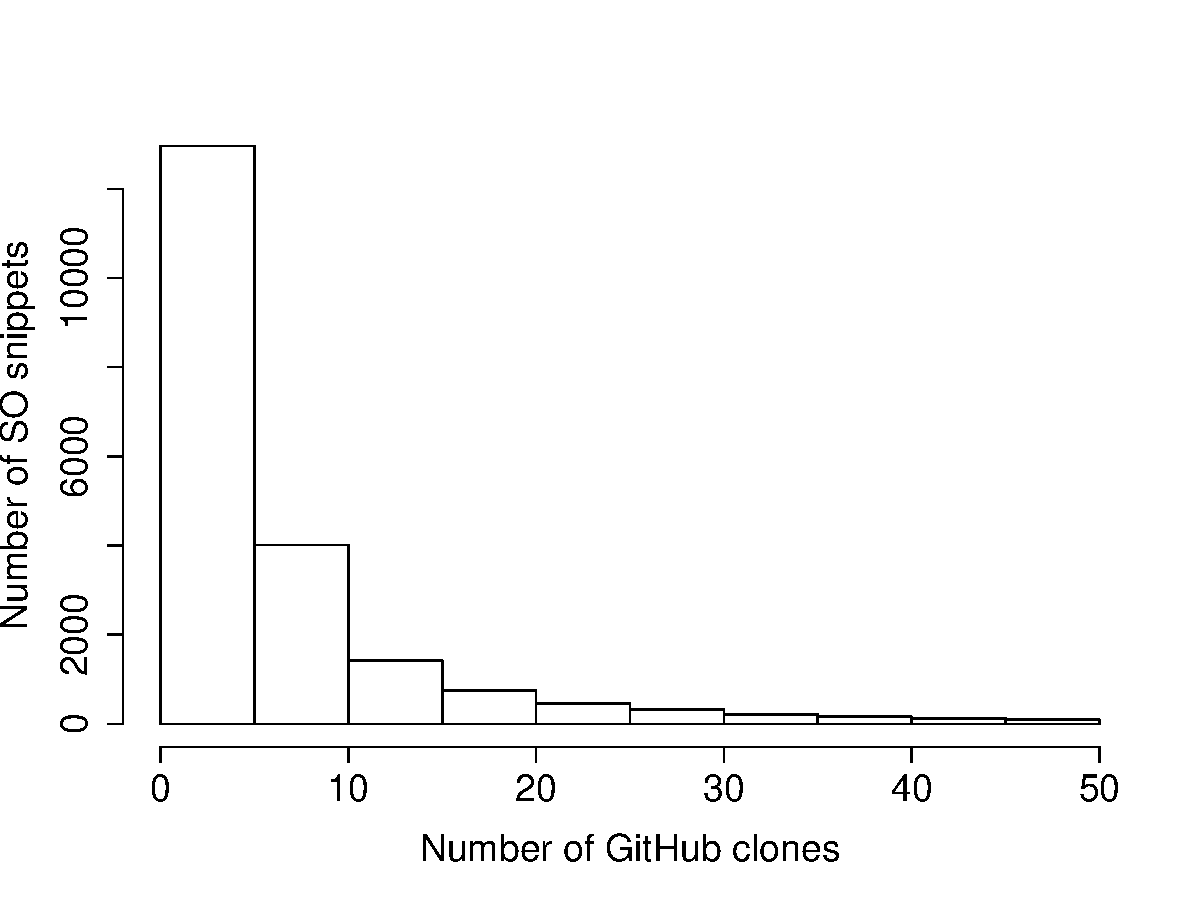
\includegraphics[scale=0.4]{figures/dist-gh-clone.pdf}
	\caption{Distribution of number of GitHub clones}
	\label{fig:num-clone}
\end{figure}

We collect the original GitHub files which contain these similar counterparts Then we extract all co-occurred methods from these GitHub files and treat them as candidate related code fragments. For each candidate in each GitHub file, we cluster its similar counterparts from other files. We keep only the clusters with size of at least two and return the remaining clusters in descending order of size.

For 11,110 out of 21K SO queries, {\tool} can retrieve related code fragments from GitHub. That is, using our SO query code base and GitHub search code corpus, {\tool} can recommend related code for 52.4\% of the queries. The SO queries have a median of 24 recommended related methods in GitHub and a mean of 74 recommended related methods. The related methods have a median of 12 average lines of code, and a mean of 14 average lines of code. The distribution of number of related methods and distribution of average lines of code are shown in Figure \ref{fig:num-related} and \ref{fig:avg-loc} respectively.

From the figures we can see that a SO query most commonly have less than ten recommendations for related code fragments, and most of the SO queries have less than 50 related methods in GitHub. Most related methods for a query will have five to thirty average lines of code.

\begin{figure}
	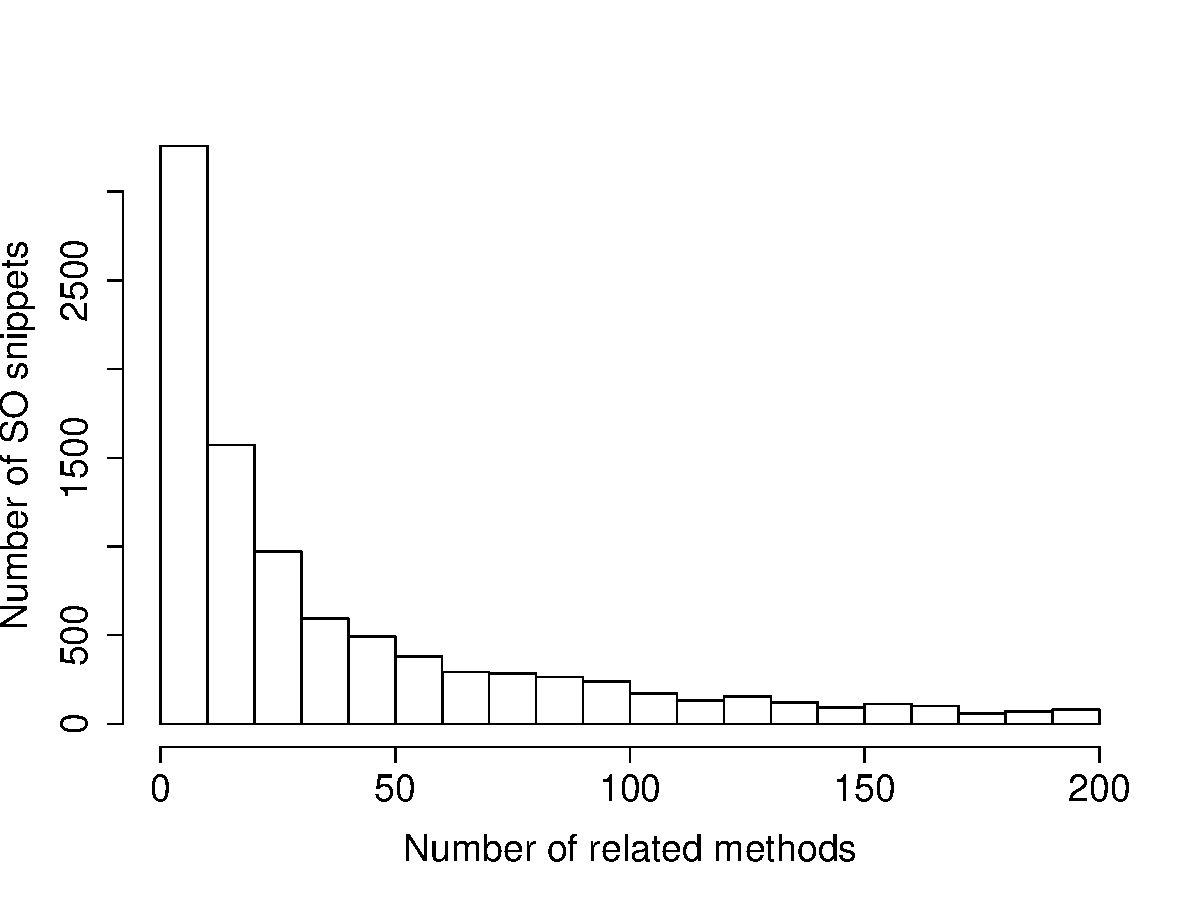
\includegraphics[scale=0.4]{figures/dist-related.pdf}
	\caption{Distribution of number of related methods}
	\label{fig:num-related}
\end{figure}

\begin{figure}
	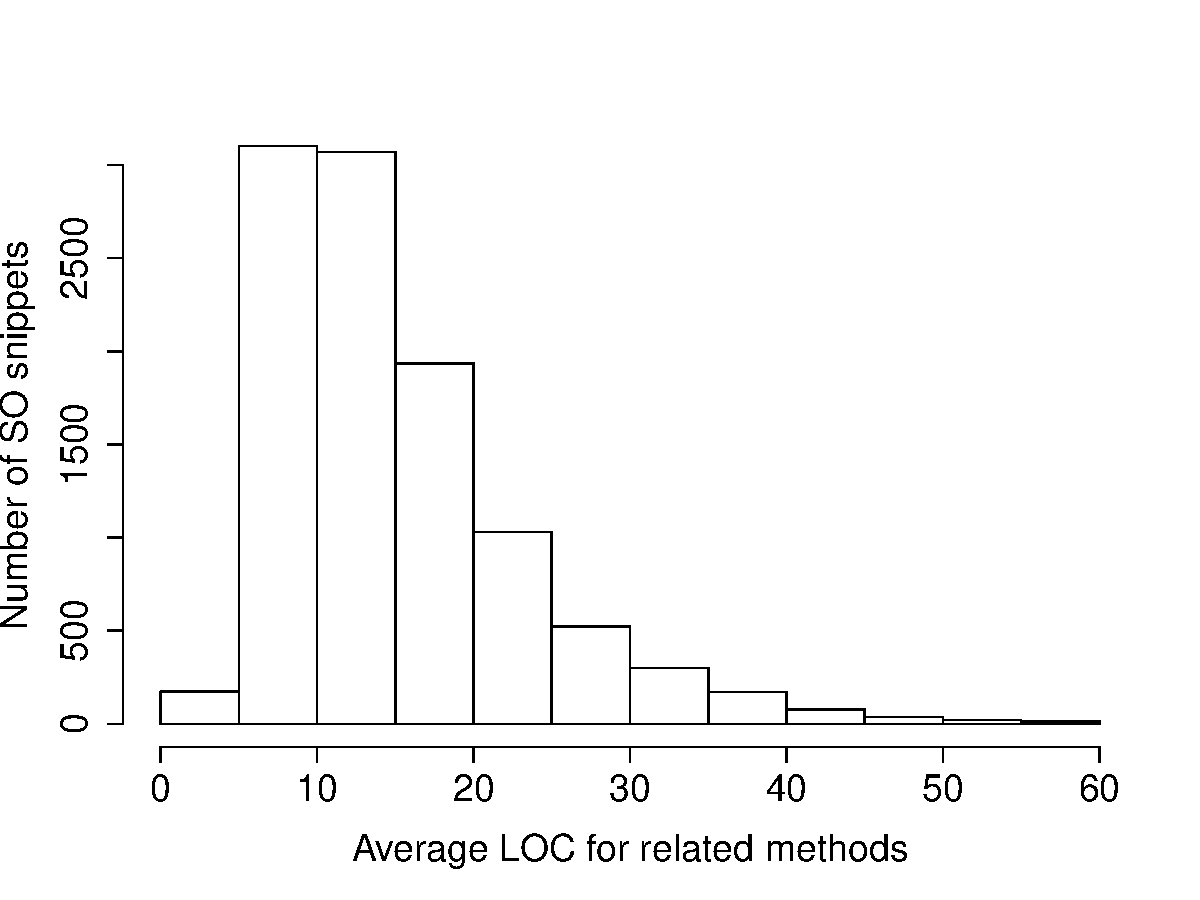
\includegraphics[scale=0.4]{figures/dist-loc.pdf}
	\caption{Distribution of average LOC of related methods}
	\label{fig:avg-loc}
\end{figure}

